\documentclass[12pt,a4paper]{article}

% ================= PACKAGES =================
\usepackage[margin=1in]{geometry}
\usepackage[T1]{fontenc}
\usepackage{graphicx}
\usepackage{titlesec}
\usepackage{tabularx}
\usepackage{longtable}
\usepackage{array}
\usepackage{hyperref}
\usepackage{xurl}
\usepackage{listings}
\usepackage{xcolor}
\usepackage{enumitem}
\usepackage{setspace}
\usepackage[most]{tcolorbox}
\usepackage{mathptmx}   % Times New Roman-equivalent font, applies to entire document

% ================= FONT SIZE LADDER =================
% Absolute sizes so nothing depends on class-relative scaling.
\newcommand{\sizeEighteen}{\fontsize{18pt}{22pt}\selectfont}  % \section
\newcommand{\sizeSixteen}{\fontsize{16pt}{20pt}\selectfont}   % \subsection
\newcommand{\sizeFourteen}{\fontsize{14pt}{17pt}\selectfont}  % \subsubsection
\newcommand{\sizeTwelve}{\fontsize{12pt}{14.5pt}\selectfont}  % body / minimum

% ================= HEADER COLORS =================
\definecolor{RamaiahBlue}{RGB}{27,31,92}
\definecolor{RamaiahMaroon}{RGB}{139,30,63}

% ================= CODE LISTING STYLE =================
% basicstyle and numberstyle both forced to 12pt -- nothing prints smaller.
% xleftmargin keeps the 12pt line numbers inside the A4 text block.
\lstdefinestyle{codestyle}{
    backgroundcolor=\color{black!5},
    commentstyle=\color{green!50!black},
    keywordstyle=\color{blue},
    stringstyle=\color{orange},
    basicstyle=\ttfamily\fontsize{12pt}{14.4pt}\selectfont,
    numberstyle=\ttfamily\fontsize{12pt}{14.4pt}\selectfont,
    breaklines=true,
    breakatwhitespace=false,
    frame=single,
    numbers=left,
    numbersep=8pt,
    xleftmargin=3.2em,
    aboveskip=10pt,
    belowskip=10pt,
    showstringspaces=false
}
\lstset{style=codestyle,columns=fullflexible,keepspaces=true}

% ================= HEADING FORMATS =================
\titleformat{\section}{\sizeEighteen\bfseries}{\thesection}{1em}{}
\titleformat{\subsection}{\sizeSixteen\bfseries}{\thesubsection}{1em}{}
\titleformat{\subsubsection}{\sizeFourteen\bfseries}{\thesubsubsection}{1em}{}

\titlespacing*{\section}{0pt}{18pt}{10pt}
\titlespacing*{\subsection}{0pt}{16pt}{8pt}
\titlespacing*{\subsubsection}{0pt}{14pt}{7pt}

% ================= REPEATABLE HEADER BANNER =================
\newcommand{\reportheader}{%
\noindent
\begin{minipage}[c]{0.42\textwidth}
  
\includegraphics[height=1.2cm]{ramaiah_logo.jpg}
\end{minipage}%
\begin{minipage}[c]{0.62\textwidth}
  \raggedleft
  {\color{RamaiahBlue}\sizeFourteen\bfseries Department of CSE (Artificial Intelligence \& Machine Learning) and CSE (Cyber Security)}
\end{minipage}\\[0.2cm]
\noindent\textcolor{RamaiahMaroon}{\rule{\linewidth}{1.2pt}}
\vspace{0.4cm}
}


\graphicspath{{../evidence/}{./}}
\hypersetup{pdfauthor={Sourav Kumar Sahu},
pdftitle={DevOps Self Learning Activity Report - Quote API},
breaklinks=true}
\begin{document}
\pagestyle{empty}
\sizeTwelve

\reportheader

\vspace{1.0cm}
\begin{center}
{\sizeEighteen \bfseries SELF LEARNING ACTIVITY REPORT \par}

\vspace{1.2cm}

{\sizeTwelve Submitted in partial fulfilment of the Requirements for \\[0.2cm]
the Academics of 5\textsuperscript{th} Semester, B.E in CSE (Cyber Security) \par}

\vspace{1.2cm}

{\sizeEighteen \bfseries DEVOPS \par}

\vspace{0.5cm}

{\sizeSixteen \bfseries 24CYAEC59 \par}

\vspace{1.2cm}

{\sizeTwelve In \par}

\vspace{0.45cm}

{\sizeFourteen \bfseries Dept. of CSE (CYBER SECURITY) \par}

\vspace{1.2cm}

{\sizeTwelve By \par}

\vspace{0.4cm}

{\sizeFourteen \bfseries USN: 1MS24CY063 \par}

\vspace{1.5cm}

{\sizeTwelve Under the guidance of \par}
\vspace{0.3cm}

{\sizeFourteen \bfseries Mr. Prashanth Reddy C \par}
\vspace{0.15cm}

{\sizeTwelve Senior Lecturer \par}
{\sizeTwelve Department of CSE (AI \& ML) and CSE (Cyber Security) \par}

\vspace{1.5cm}

{\sizeSixteen \bfseries M. S. Ramaiah Institute of Technology \par}
\vspace{0.3cm}
{\sizeTwelve (Autonomous Institute Affiliated to VTU) \\ MSR Nagar, MSRIT Post \par}
\vspace{0.1cm}
{\sizeTwelve Bangalore-560054, Karnataka, India \par}
\end{center}

\newpage

% ======================================================

\reportheader

\vspace{1.0cm}
\begin{center}
{\sizeEighteen \bfseries Certificate \par}
\end{center}

\vspace{0.8cm}

\noindent
{\sizeTwelve
This is to certify that the work carried out is a bonafide record of the project based learning activity work on the DevOps course done by Sourav Kumar Sahu (1MS24CY063) under my supervision and guidance, in partial fulfilment of the requirements for the award of the Bachelor of Engineering in Computer Science \& Engineering (Cyber Security) from Ramaiah Institute of Technology, Bangalore for the academic year 2026-2027.
\par}

\vspace{3.5cm}

\noindent
{\sizeTwelve Candidate Sign \hfill Faculty Sign \par}

\newpage
\pagestyle{plain}

% ======================================================

\section*{LIST OF PROJECT BASED LEARNING COMPONENTS}

\noindent
{\sizeTwelve
\textbf{COURSE NAME:} DevOps \hfill \textbf{COURSE CODE:} 24CYAEC59 \\
\textbf{CREDITS:} 1:0:0 \hfill \textbf{CONTACT HOURS:} 15L \\
\textbf{MAX. MARKS:} 20
\par}

\vspace{0.6cm}

{\sizeTwelve
\setlength{\tabcolsep}{4pt}
\renewcommand{\arraystretch}{1.25}
\begin{longtable}{|>{\centering\arraybackslash}m{1.2cm}|>{\raggedright\arraybackslash}p{10.6cm}|>{\centering\arraybackslash}m{1.8cm}|}
\hline
\multicolumn{1}{|c|}{\textbf{Sl. No}} &
\multicolumn{1}{c|}{\textbf{Description}} &
\multicolumn{1}{c|}{\textbf{Marks}} \\
\hline
\endhead

1 &
\textbf{CI/CD Pipeline using Git, Maven/Gradle and Jenkins.}
Set up a version-controlled build pipeline for a sample application. Create a Git repository, use feature branching and merging, configure a Maven or Gradle build with dependency management, integrate the project into a Jenkins job that pulls from Source Code Management (SCM), triggers automatically on commit, executes the build, performs a post-build action, and add one CI-related enhancement (automated tests, build versioning, or GitHub Actions).

\textit{Covers: Unit 1 (DevOps culture/pipeline), Unit 2 (Git, Maven/Gradle), Unit 3 (Jenkins CI). Maps to CO1, CO2, CO3.}
& 10 \\
\hline

2 &
\textbf{Configuration Management with Ansible and Deployment on Kubernetes.}
Write an Ansible playbook (using variables, handlers, and at least one role) to configure and deploy the application built in Component 1. Containerize the application and write Kubernetes manifests (Deployment, Service, and a ConfigMap/PVC where applicable). Deploy on a local cluster (Minikube/Kind), demonstrate scaling using replica sets, show the use of labels and selectors, and add one deployment-related enhancement (rollback, ConfigMap, probes, multi-stage Dockerfile, second microservice, or health endpoint).

\textit{Covers: Unit 4 (Ansible), Unit 5 (Kubernetes). Maps to CO4, CO5.}
& 10 \\
\hline

\end{longtable}
\par}

\newpage

% ======================================================
% ASSESSMENT RUBRICS
% ======================================================
\section*{Assessment Rubrics}
{\sizeTwelve Evaluation for \textbf{each} 10-mark component will be based on the following rubrics.\par}

\vspace{0.4cm}

{\sizeTwelve
\setlength{\tabcolsep}{4pt}
\renewcommand{\arraystretch}{1.25}
\begin{longtable}{|>{\raggedright\arraybackslash}p{3.0cm}|>{\raggedright\arraybackslash}p{3.5cm}|>{\raggedright\arraybackslash}p{3.5cm}|>{\raggedright\arraybackslash}p{3.5cm}|}
\hline

\textbf{Criteria} & \textbf{2 --- Good} & \textbf{1 --- Average} & \textbf{0 --- Poor} \\

\hline
\endhead
Concept Understanding (2 marks) & Answers ``why'' questions correctly and immediately (e.g., webhook vs.\ polling, what a handler does, Deployment vs.\ ReplicaSet, why the chosen enhancement matters) & Gets the basic idea right but stumbles on follow-up questions or confuses related concepts & Cannot explain own pipeline; answers suggest it was copied or AI-generated without understanding \\
\hline
Core Implementation (2 marks) & Required pipeline (Git+Jenkins for Comp.\ 1 / Ansible+K8s+scaling for Comp.\ 2) runs end-to-end live, without intervention & Works but needs manual triggering, a workaround, or partial failure & Doesn't run at all during the demo; only screenshots are shown \\
\hline
Enhancement (2 marks) & At least one enhancement from Section 3/4's list implemented and demonstrated live, working correctly & Enhancement attempted but incomplete, or only explained without being runnable & No enhancement attempted \\
\hline
Analysis \& Interpretation (2 marks) & Explains build logs, scaling behaviour, or enhancement outcomes in own words; interprets output unprompted & Describes what happened but not why, or needs prompting to interpret output & No interpretation offered; treats commands as a checklist \\
\hline
Documentation \& Presentation (2 marks) & Report fully personalized  and confidently walks through the pipeline unprompted & Mostly complete report or needs guidance/prompting during the demo & Unedited template, mismatched screenshots, or cannot navigate own setup \\
\hline
\end{longtable}
\par}

\newpage

% ======================================================
% MARKS AWARDED TABLE
% ======================================================
\section*{Marks Awarded}

\vspace{0.3cm}

{\sizeTwelve
\setlength{\tabcolsep}{3pt}
\renewcommand{\arraystretch}{1.5}
\begin{longtable}{|>{\centering\arraybackslash}p{1.0cm}|>{\raggedright\arraybackslash}p{2.2cm}|>{\raggedright\arraybackslash}p{2.2cm}|>{\raggedright\arraybackslash}p{2.0cm}|>{\raggedright\arraybackslash}p{2.3cm}|>{\raggedright\arraybackslash}p{2.5cm}|>{\centering\arraybackslash}p{1.4cm}|}
\hline
\textbf{Sl. No} &
\textbf{Concept Under- standing (2)} &
\textbf{Core Imple- mentation (2)} &
\textbf{Enhance- ment (2)} &
\textbf{Analysis \& Interpre- tation (2)} &
\textbf{Documen- tation \& Presenta- tion (2)} &
\textbf{Total} \\
\hline
\parbox[c][1.1cm][c]{1.0cm}{\centering 1} & & & & & & \\
\hline
\parbox[c][1.1cm][c]{1.0cm}{\centering 2} & & & & & & \\
\hline
\multicolumn{6}{|c|}{\parbox[c][1.1cm][c]{13.0cm}{\centering\textbf{TOTAL MARKS}}} &
\parbox[c][1.1cm][c]{1.4cm}{\centering} \\
\hline
\end{longtable}
\par}

\newpage

% ======================================================

\emergencystretch=2em

\section*{Component 1: CI/CD Pipeline using Git, Maven/Gradle and Jenkins}

\subsection*{Abstract}
The Quote API is a small Java service that returns a list of quotes, a random quote and a health response. Its source is stored on GitHub, built with Maven and checked by Jenkins through an automatic SCM polling trigger. Three JUnit tests run before packaging, and a successful build archives the executable JAR for the deployment component.

\subsection*{Introduction}
DevOps relies on tight integration between development and operations, and Continuous Integration is one of its foundational practices. Git provides distributed version control so multiple developers can work on branches without conflicts. Maven and Gradle automate the build lifecycle --- compiling code, managing dependencies, and packaging artifacts --- removing the need for manual, error-prone build steps. Jenkins ties these together by automatically triggering a build whenever new code is pushed, giving teams fast feedback on whether the codebase is in a working state. This component walks through setting up all three in a single working pipeline.

This project uses Java 17, Spring Boot and Maven for the Quote API. There is no database or frontend: the three routes are \texttt{/quotes}, \texttt{/quotes/random} and \texttt{/health}. The source repository for both components is \url{https://github.com/printf-sourav/DevOps-project}.

\subsection*{Implementation}
\subsubsection*{Development Environment}
\begin{itemize}[nosep]
\item Local system: Windows 11 with Ubuntu 26.04.1 LTS under WSL2, using Linux kernel 6.6.87.2.
\item Git: 2.55.0.windows.3 locally and 2.53.0 in Ubuntu.
\item Application build: Microsoft OpenJDK 17.0.20 and Maven 3.9.11 on Windows.
\item Jenkins agent: OpenJDK 21.0.12.1 and Maven 3.9.12 in Ubuntu; the project still targets Java 17 bytecode.
\item Jenkins: 2.580.2 LTS, with Pipeline, Git, JUnit and Timestamper plugins.
\item Application: Spring Boot 3.5.16, with Spring Web and Spring Boot Test dependencies.
\end{itemize}

\paragraph{Application code.}
The controller below is the actual repository source. Its immutable list avoids storage setup and shared mutable state, which keeps the pipeline demonstration focused on the DevOps tools.

\begin{lstlisting}[language={Java}]
package io.github.printfsourav.quotes;

import java.util.List;
import java.util.Map;
import java.util.concurrent.ThreadLocalRandom;
import org.springframework.web.bind.annotation.GetMapping;
import org.springframework.web.bind.annotation.RestController;

@RestController
public class QuoteController {
    public record Quote(int id, String text) {}

    private final List<Quote> quotes = List.of(
        new Quote(1, "Start small. Keep improving."),
        new Quote(2, "Build it, test it, then ship it."),
        new Quote(3, "A little progress every day adds up.")
    );

    @GetMapping("/quotes")
    public List<Quote> list() {
        return quotes;
    }

    @GetMapping("/quotes/random")
    public Quote random() {
        return quotes.get(ThreadLocalRandom.current().nextInt(quotes.size()));
    }

    @GetMapping("/health")
    public Map<String, String> health() {
        return Map.of("status", "UP");
    }
}
\end{lstlisting}


\subsubsection*{Step 1: Git Repository and Branching}
The repository was initially empty. A small setup commit was created on \texttt{main}, followed by the application and pipeline commits on \texttt{feature/quote-pipeline}. Both branches remain on GitHub. Merge commit \texttt{1956418} joins the feature branch into main, so the history demonstrates branching and merging rather than a single upload.

The following excerpt shows the branch and commit names used in the project; the other focused pipeline commits are visible in the Results graph.

\begin{lstlisting}[language={bash}]
git clone https://github.com/printf-sourav/DevOps-project.git .
git switch -c feature/quote-pipeline
git add pom.xml src
git commit -m "Add a quote API with three endpoints and tests"
git switch main
git merge --no-ff feature/quote-pipeline -m "Merge the quote API and its build and deployment pipeline"
git push origin main feature/quote-pipeline
git log --graph --oneline --all
\end{lstlisting}


\subsubsection*{Step 2: Maven Build Configuration (pom.xml excerpt)}
The complete Maven configuration is shown below. The parent manages compatible dependency and plugin versions; \texttt{java.version} selects Java 17, and the Spring Boot plugin creates an executable JAR named \texttt{target/quote-api.jar}.

\begin{lstlisting}[language={XML}]
<?xml version="1.0" encoding="UTF-8"?>
<project xmlns="http://maven.apache.org/POM/4.0.0"
         xmlns:xsi="http://www.w3.org/2001/XMLSchema-instance"
         xsi:schemaLocation="http://maven.apache.org/POM/4.0.0 https://maven.apache.org/xsd/maven-4.0.0.xsd">
  <modelVersion>4.0.0</modelVersion>
  <parent>
    <groupId>org.springframework.boot</groupId>
    <artifactId>spring-boot-starter-parent</artifactId>
    <version>3.5.16</version>
    <relativePath/>
  </parent>
  <groupId>io.github.printfsourav</groupId>
  <artifactId>quote-api</artifactId>
  <version>1.0.0</version>
  <name>Quote API</name>
  <description>A small REST API for a DevOps pipeline assignment</description>
  <properties>
    <java.version>17</java.version>
  </properties>
  <dependencies>
    <dependency>
      <groupId>org.springframework.boot</groupId>
      <artifactId>spring-boot-starter-web</artifactId>
    </dependency>
    <dependency>
      <groupId>org.springframework.boot</groupId>
      <artifactId>spring-boot-starter-test</artifactId>
      <scope>test</scope>
    </dependency>
  </dependencies>
  <build>
    <finalName>quote-api</finalName>
    <plugins>
      <plugin>
        <groupId>org.springframework.boot</groupId>
        <artifactId>spring-boot-maven-plugin</artifactId>
      </plugin>
    </plugins>
  </build>
</project>
\end{lstlisting}

\begin{lstlisting}[language={bash}]
mvn clean package
java -jar target/quote-api.jar
# Run these requests in another terminal.
curl http://localhost:8080/health
curl http://localhost:8080/quotes
curl http://localhost:8080/quotes/random
\end{lstlisting}


\subsubsection*{Step 3: Jenkins Pipeline (Jenkinsfile)}
The Jenkins job uses \textbf{Pipeline script from SCM}, Git repository \url{https://github.com/printf-sourav/DevOps-project.git}, branch \texttt{*/main}, and script path \texttt{Jenkinsfile}. Declarative Pipeline checks out that SCM automatically. The first manual run registers the polling trigger; later changes are picked up every minute without pressing Build Now.

The Test stage must pass before Build starts. Test results are published as JUnit XML, and the Build stage archives the JAR with a fingerprint. The Windows/Linux command branches let the same file work on either type of build agent.

\par\noindent\begin{minipage}{\linewidth}
\begin{lstlisting}[language={}]
pipeline {
    agent any
    options {
        timestamps()
        disableConcurrentBuilds()
        buildDiscarder(logRotator(numToKeepStr: '10'))
    }
    triggers { pollSCM('* * * * *') }
    stages {
        stage('Test') {
            steps {
                script {
                    if (isUnix()) { sh 'mvn -B clean test' }
                    else { bat 'mvn -B clean test' }
                }
            }
            post { always { junit 'target/surefire-reports/*.xml' } }
        }
        stage('Build') {
            steps {
                script {
                    if (isUnix()) { sh 'mvn -B -DskipTests package' }
                    else { bat 'mvn -B -DskipTests package' }
                }
                archiveArtifacts artifacts: 'target/quote-api.jar', fingerprint: true
            }
        }
    }
}
\end{lstlisting}
\end{minipage}\par


\subsubsection*{Step 4: CI Enhancement}
The chosen enhancement is \textbf{automated tests in CI}. Three tests verify the fixed quote list, check that the random route returns a quote from that list, and verify the health response. MockMvc exercises the controller's HTTP mappings and JSON output without requiring a separate server process. This was chosen because it checks meaningful behaviour with little extra setup.

\begin{lstlisting}[language={Java}]
package io.github.printfsourav.quotes;

import static org.hamcrest.Matchers.hasSize;
import static org.junit.jupiter.api.Assertions.assertTrue;
import static org.springframework.test.web.servlet.request.MockMvcRequestBuilders.get;
import static org.springframework.test.web.servlet.result.MockMvcResultMatchers.jsonPath;
import static org.springframework.test.web.servlet.result.MockMvcResultMatchers.status;

import com.fasterxml.jackson.databind.ObjectMapper;
import org.junit.jupiter.api.Test;
import org.springframework.beans.factory.annotation.Autowired;
import org.springframework.boot.test.autoconfigure.web.servlet.WebMvcTest;
import org.springframework.test.web.servlet.MockMvc;

@WebMvcTest(QuoteController.class)
class QuoteControllerTest {
    @Autowired private MockMvc mvc;
    @Autowired private ObjectMapper mapper;

    @Test
    void listsTheThreeQuotes() throws Exception {
        mvc.perform(get("/quotes"))
            .andExpect(status().isOk())
            .andExpect(jsonPath("$", hasSize(3)))
            .andExpect(jsonPath("$[0].text").value("Start small. Keep improving."));
    }

    @Test
    void randomQuoteBelongsToTheList() throws Exception {
        var controller = new QuoteController();
        for (int i = 0; i < 20; i++) {
            var response = mvc.perform(get("/quotes/random"))
                .andExpect(status().isOk()).andReturn();
            var quote = mapper.readValue(response.getResponse().getContentAsString(),
                QuoteController.Quote.class);
            assertTrue(controller.list().contains(quote));
        }
    }

    @Test
    void healthEndpointIsReadyForProbes() throws Exception {
        mvc.perform(get("/health"))
            .andExpect(status().isOk())
            .andExpect(jsonPath("$.status").value("UP"));
    }
}
\end{lstlisting}


\subsubsection*{Description of the Activity}
The local Maven build and API requests were checked before Jenkins was configured. This separated application problems from CI environment problems. The first Jenkins build could start Java but could not compile the application because the Ubuntu setup had only a runtime. Installing the full JDK supplied the compiler, and the next run passed.

Jenkins also loaded plugins slowly when its home directory was on the Windows-mounted filesystem. Moving that directory to Ubuntu's native filesystem allowed initialization to finish quickly. These were environment fixes; the API did not need additional features to solve them.

After the working run, a documentation commit was pushed to main. Jenkins build \#3 recorded \textbf{Started by an SCM change}, completed in about 72 seconds, published three passed tests and archived \texttt{quote-api.jar}. This distinguishes an actual automatic CI run from the initial manual setup run. Polling was chosen instead of a webhook so the local server did not need a public URL.

To check that the tests could catch a regression, the health status was temporarily changed from UP to DOWN. The health test failed. The original source was restored, and the final local build passed all three tests. In the pipeline, \texttt{-DskipTests} is used only in the packaging stage because the preceding stage has already tested the same checked-out source.

\subsection*{Results}
The local build reported three tests with zero failures, errors or skipped tests. The automatically triggered Jenkins run completed with SUCCESS and provided the archived JAR. The figures below combine direct Jenkins browser screenshots with clearly labelled renderings of actual recorded command output; the original logs are stored in the repository's \texttt{reports/evidence} directory.

\clearpage
\begin{center}
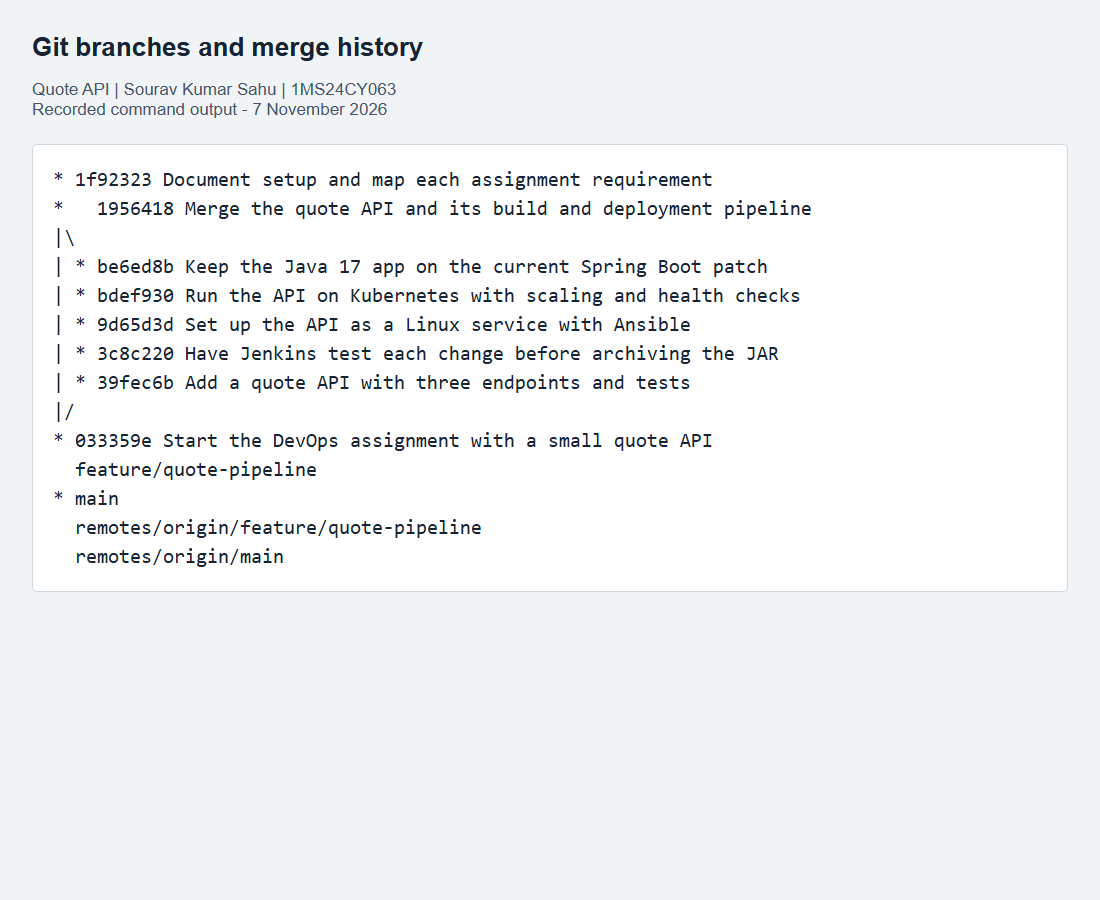
\includegraphics[width=\linewidth,height=0.78\textheight,keepaspectratio]{git-history.png}
\end{center}
\noindent Git history: main and feature/quote-pipeline are retained, and the merge commit is visible.

\clearpage
\begin{center}
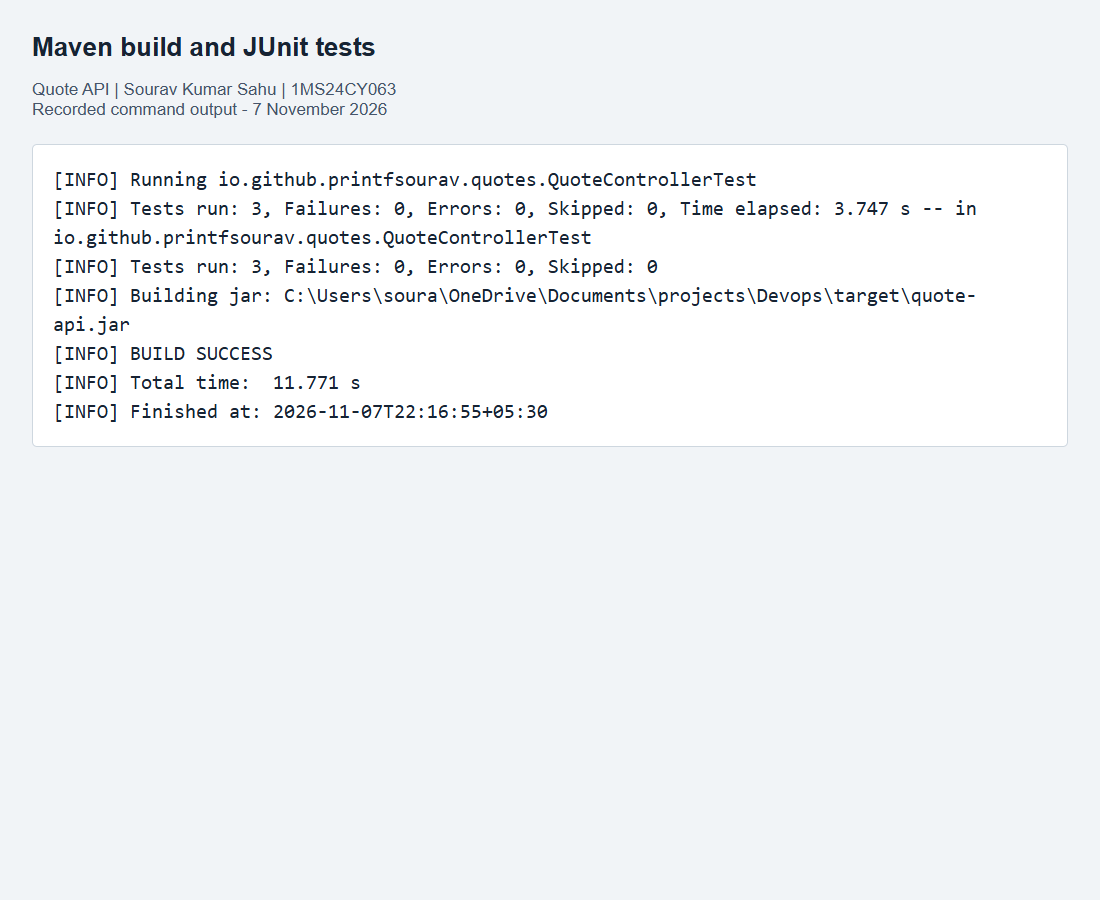
\includegraphics[width=\linewidth,height=0.78\textheight,keepaspectratio]{maven-build.png}
\end{center}
\noindent Local Maven result: all three tests passed and the executable JAR was packaged successfully.

\clearpage
\begin{center}
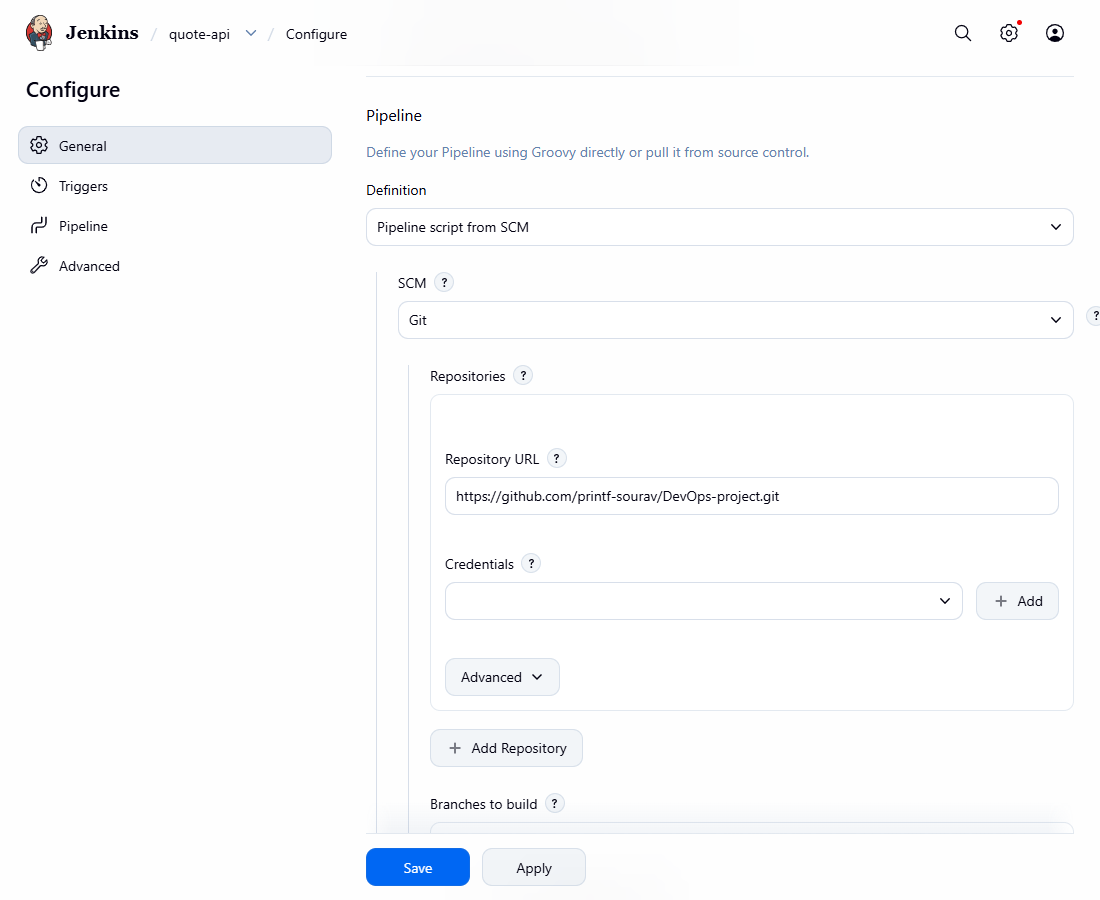
\includegraphics[width=\linewidth,height=0.78\textheight,keepaspectratio]{jenkins-config.png}
\end{center}
\noindent Jenkins SCM configuration: the Pipeline job reads from the actual project repository.

\clearpage
\begin{center}
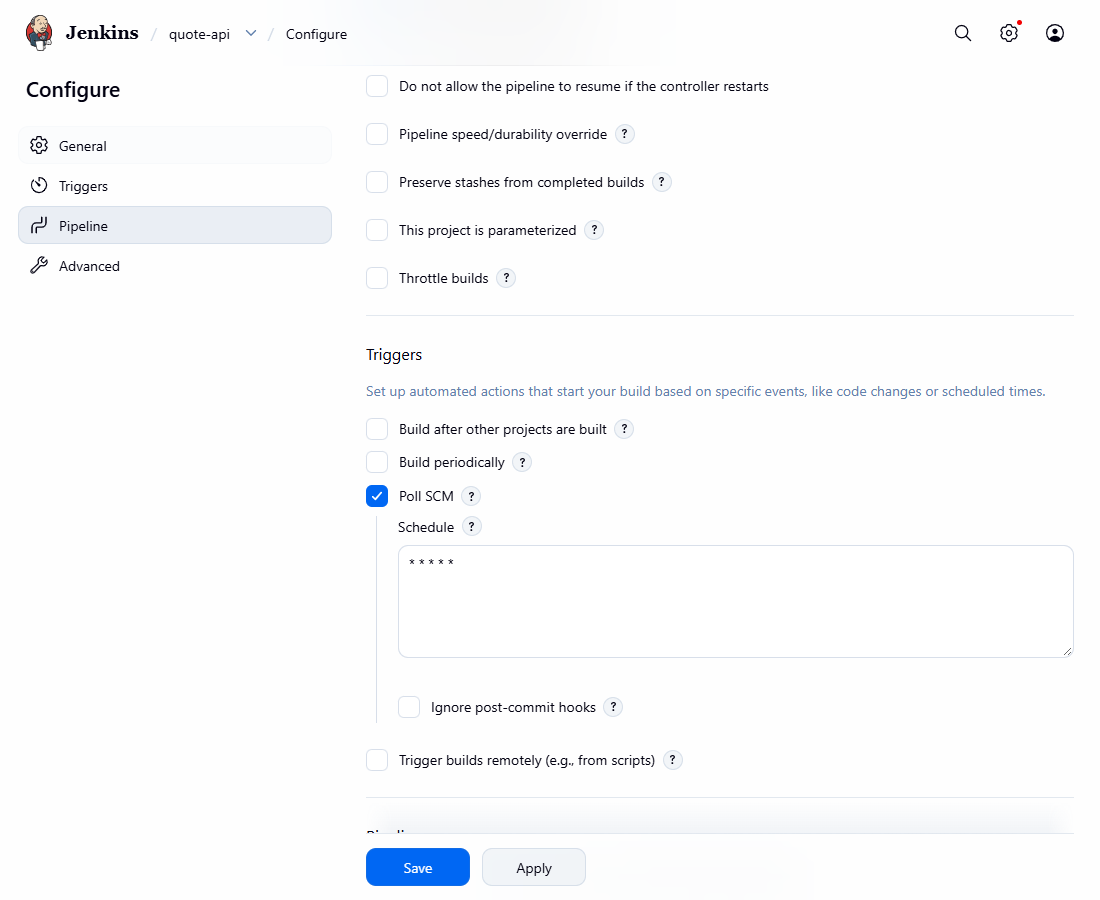
\includegraphics[width=\linewidth,height=0.78\textheight,keepaspectratio]{jenkins-trigger.png}
\end{center}
\noindent Jenkins trigger: Poll SCM is enabled with a one-minute schedule.

\clearpage
\begin{center}
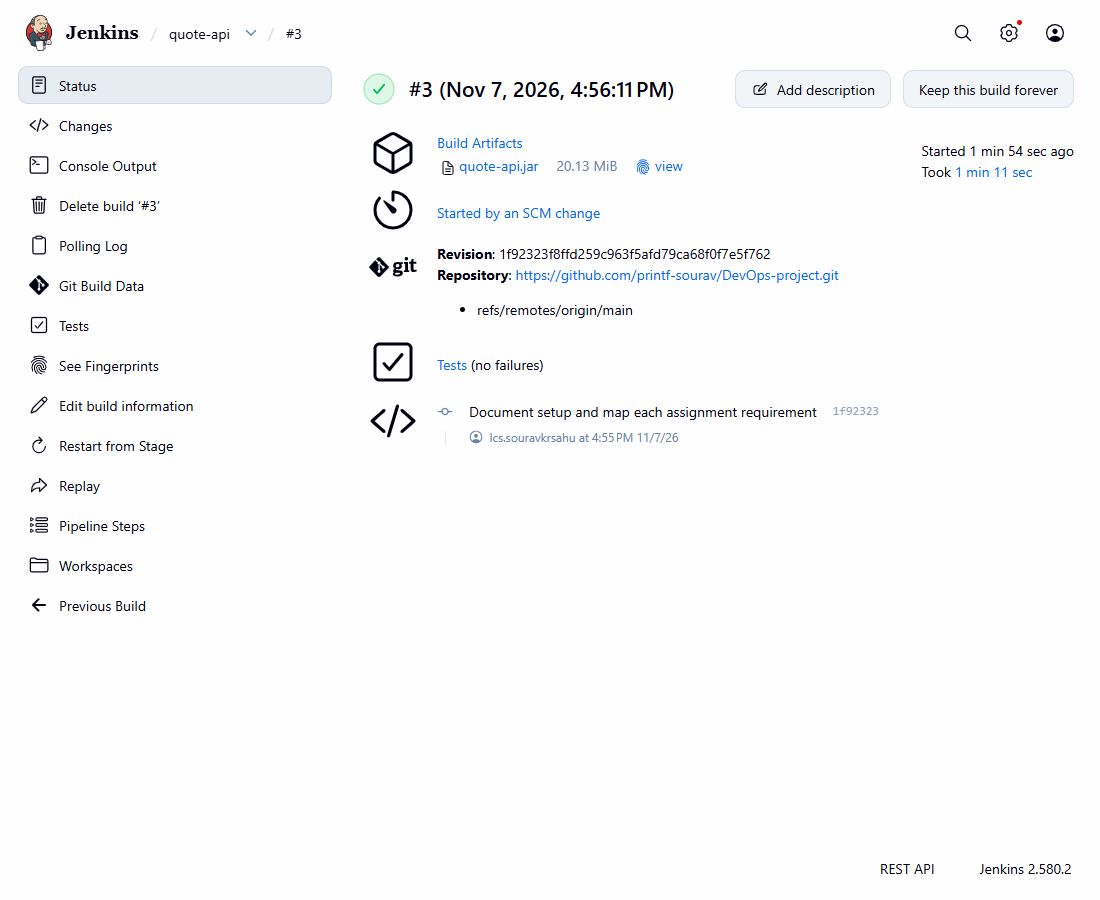
\includegraphics[width=\linewidth,height=0.78\textheight,keepaspectratio]{jenkins-build.png}
\end{center}
\noindent Jenkins build \#3: SUCCESS, an SCM-change cause, no test failures and the archived quote-api.jar artifact.

\clearpage
\begin{center}
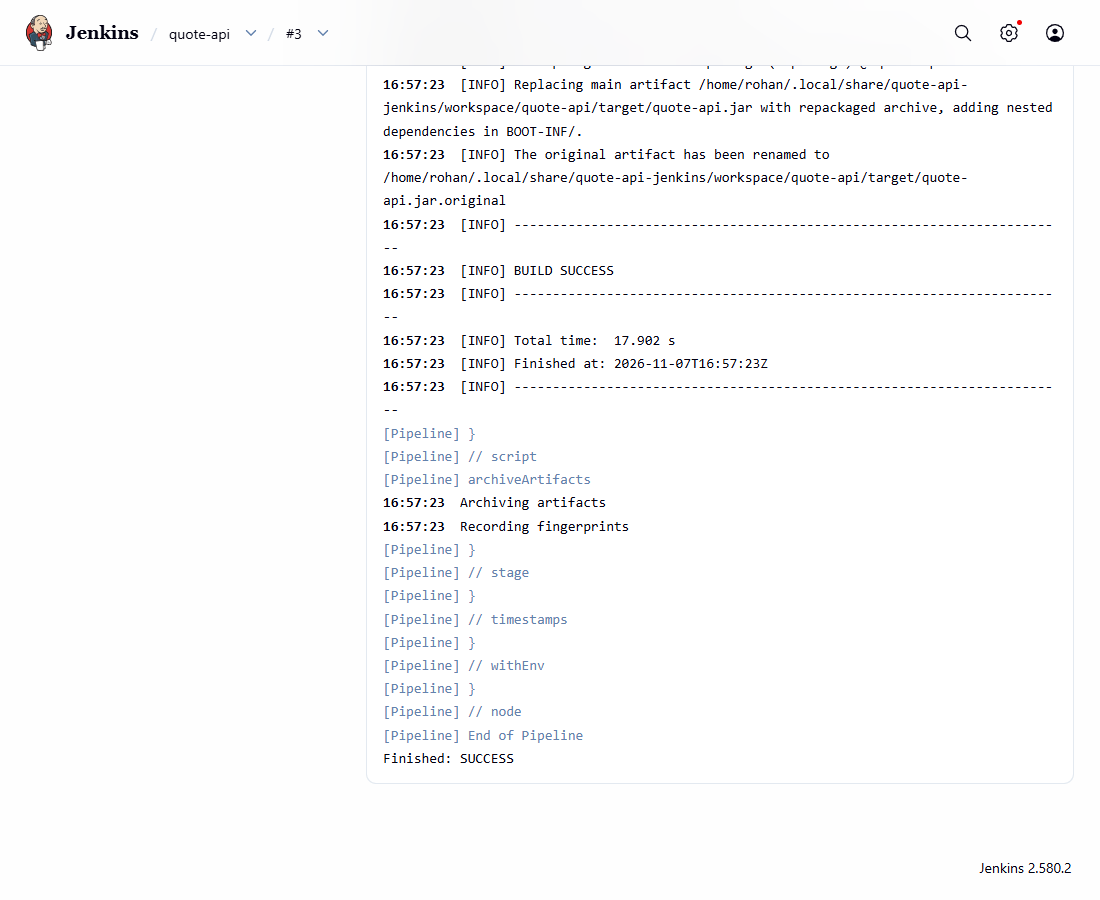
\includegraphics[width=\linewidth,height=0.78\textheight,keepaspectratio]{jenkins-console.png}
\end{center}
\noindent Jenkins console: Maven BUILD SUCCESS is followed by artifact archiving and fingerprint recording.

\clearpage
\begin{center}
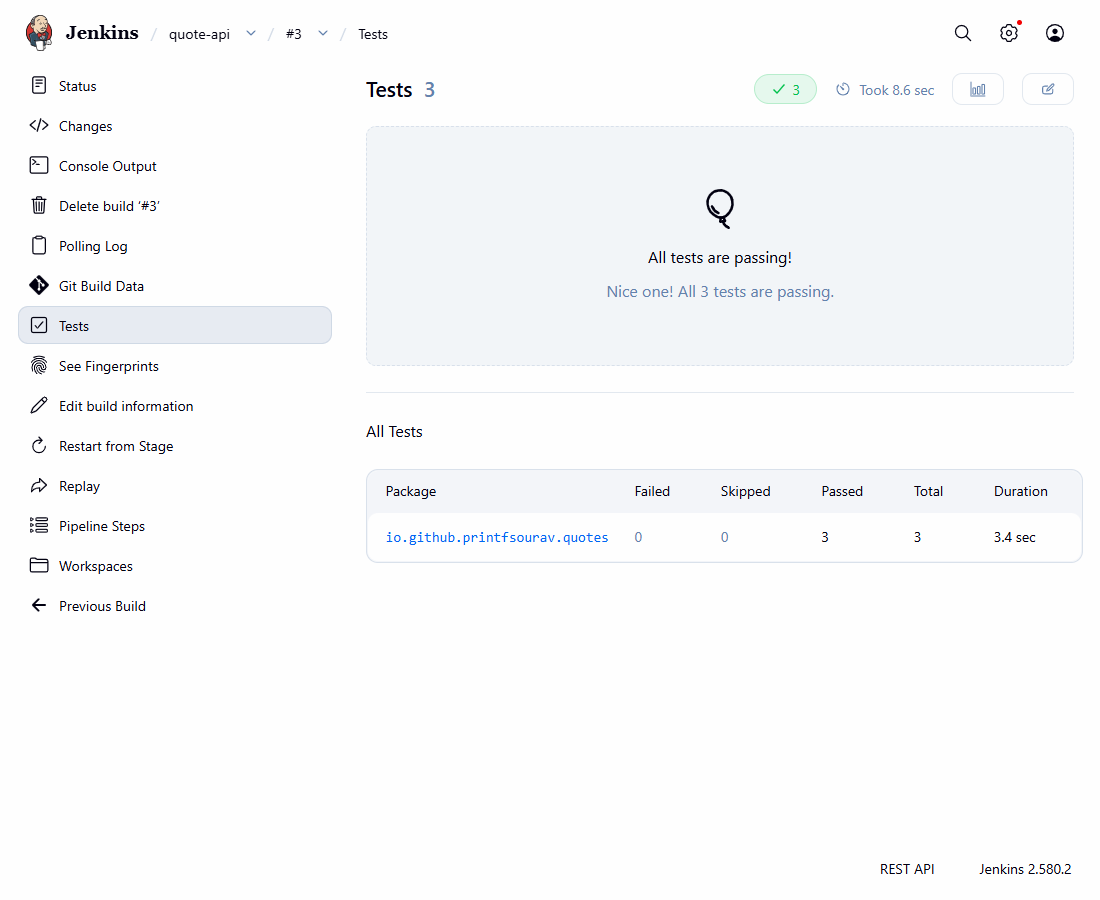
\includegraphics[width=\linewidth,height=0.78\textheight,keepaspectratio]{jenkins-tests.png}
\end{center}
\noindent CI enhancement: Jenkins publishes the three passing JUnit tests.


\subsection*{Conclusion}
The project connects a Git change to a tested, runnable artifact through Jenkins. The failed health-response check showed why tests should run before packaging, while the SCM-change build demonstrated that the checks no longer depend on a manual trigger. Keeping the API small made the build and environment failures easier to understand.

\newpage
\section*{Component 2: Configuration Management with Ansible and Deployment on Kubernetes}

\subsection*{Abstract}
This component deploys the same Quote API from Component 1 as a Linux service and as a containerized Kubernetes workload. An Ansible role installs Java, copies the built JAR and manages a systemd service, while Docker packages the application for a local Kind cluster. The deployment was scaled from three to five healthy replicas and back to three, with HTTP health probes as the deployment enhancement.

\subsection*{Introduction}
Once code is built, it must be reliably deployed and run at scale. Ansible is an agentless configuration management tool that uses YAML playbooks to describe the desired state of a server (installed packages, files, running services), making infrastructure changes repeatable and version-controlled. Kubernetes takes this further by orchestrating containerized applications across a cluster, automatically handling scheduling, scaling, networking, and self-healing. This component demonstrates both: using Ansible to configure a host, and Kubernetes to run and scale the containerized application.

The managed host is the local Ubuntu WSL system with systemd. A dedicated Kind cluster named \texttt{quote-demo} runs the containerized service. Both deployments use the Maven-built Quote API JAR from \url{https://github.com/printf-sourav/DevOps-project}; neither requires a database, PVC or paid cloud service.

\subsection*{Implementation}
\subsubsection*{Development Environment}
\begin{itemize}[nosep]
\item Control and managed host: Ubuntu 26.04.1 LTS under WSL2, with systemd.
\item Ansible Core 2.20.1; the inventory uses the local connection plugin.
\item Java 17 runtime for the installed application service.
\item Docker Engine 29.1.3 in Ubuntu WSL; Docker Desktop was unavailable during verification.
\item Kind 0.31.0, Kubernetes 1.35.0 and kubectl 1.35.0.
\item Image: \texttt{quote-api:1.0}; runtime base: \texttt{eclipse-temurin:17-jre-jammy}.
\end{itemize}

\subsubsection*{Step 1: Ansible Playbook}
The inventory below defines one actual target host. The \texttt{quote\_api} role was initialized with the Ansible Galaxy role command; only its used directories are retained in the finished repository.
\paragraph{Inventory: ansible/inventory.}

\begin{lstlisting}[language={}]
[app_servers]
localhost ansible_connection=local
\end{lstlisting}

\paragraph{Playbook: ansible/playbook.yml.}

\begin{lstlisting}[language={}]
---
- name: Configure the Quote API server
  hosts: app_servers
  become: true
  roles:
    - quote_api
\end{lstlisting}

\paragraph{Role variables: defaults/main.yml.}

\begin{lstlisting}[language={}]
---
app_port: 8081
app_directory: /opt/quote-api
app_user: quote-api
app_jar: "{{ playbook_dir }}/../target/quote-api.jar"
\end{lstlisting}


\paragraph{Role tasks: tasks/main.yml.}
The tasks install the runtime, create an unprivileged service account, copy the JAR and render the unit file. Both changed files notify the same restart handler. Flushing the handler before the health check ensures that the response comes from the newly deployed version.

\begin{lstlisting}[language={}]
---
- name: Install the Java runtime
  ansible.builtin.apt:
    name: openjdk-17-jre-headless
    state: present
    update_cache: true
    cache_valid_time: 3600

- name: Create a service account
  ansible.builtin.user:
    name: "{{ app_user }}"
    system: true
    shell: /usr/sbin/nologin
    create_home: false

- name: Create the application directory
  ansible.builtin.file:
    path: "{{ app_directory }}"
    state: directory
    owner: "{{ app_user }}"
    group: "{{ app_user }}"
    mode: '0755'

- name: Copy the built application
  ansible.builtin.copy:
    src: "{{ app_jar }}"
    dest: "{{ app_directory }}/quote-api.jar"
    owner: "{{ app_user }}"
    group: "{{ app_user }}"
    mode: '0644'
  notify: Restart quote API

- name: Install the service definition
  ansible.builtin.template:
    src: quote-api.service.j2
    dest: /etc/systemd/system/quote-api.service
    mode: '0644'
  notify: Restart quote API

- name: Apply pending service changes
  ansible.builtin.meta: flush_handlers

- name: Enable and start the service
  ansible.builtin.systemd_service:
    name: quote-api
    enabled: true
    state: started
    daemon_reload: true

- name: Wait for the API to become healthy
  ansible.builtin.uri:
    url: "http://127.0.0.1:{{ app_port }}/health"
    return_content: true
  register: health
  until: health.status == 200 and health.json.status == 'UP'
  retries: 20
  delay: 3
\end{lstlisting}

\paragraph{Restart handler: handlers/main.yml.}

\begin{lstlisting}[language={}]
---
- name: Restart quote API
  ansible.builtin.systemd_service:
    name: quote-api
    state: restarted
    daemon_reload: true
\end{lstlisting}

\paragraph{Service template: templates/quote-api.service.j2.}

\begin{lstlisting}[language={}]
[Unit]
Description=Quote API
After=network.target

[Service]
User={{ app_user }}
Group={{ app_user }}
WorkingDirectory={{ app_directory }}
Environment=APP_PORT={{ app_port }}
ExecStart=/usr/bin/java -jar {{ app_directory }}/quote-api.jar
Restart=on-failure
RestartSec=5
NoNewPrivileges=true
PrivateTmp=true
ProtectSystem=strict
ProtectHome=true
TimeoutStopSec=20

[Install]
WantedBy=multi-user.target
\end{lstlisting}

\begin{lstlisting}[language={bash}]
cd ansible
ansible-playbook -i inventory playbook.yml
curl http://localhost:8081/health
ansible-playbook -i inventory playbook.yml
\end{lstlisting}


These verification runs used root for privilege escalation. When running as a regular user without passwordless sudo, add \texttt{--ask-become-pass}. The second run checks whether the declared state is already satisfied instead of reinstalling and restarting everything.

\subsubsection*{Step 2: Dockerfile}
The Dockerfile copies the packaged artifact into a Java runtime image and runs the process as UID 10001. Maven is not installed in the runtime image. Only the built JAR enters the build context through \texttt{.dockerignore}.

\begin{lstlisting}[language={}]
FROM eclipse-temurin:17-jre-jammy
WORKDIR /app
COPY --chown=10001:10001 target/quote-api.jar app.jar
USER 10001:10001
EXPOSE 8080
ENTRYPOINT ["java", "-XX:MaxRAMPercentage=75.0", "-jar", "app.jar"]
\end{lstlisting}

\begin{lstlisting}[language={bash}]
docker build -t quote-api:1.0 .
docker run --rm --name quote-api -p 127.0.0.1:8082:8080 quote-api:1.0
# In a second terminal:
curl http://localhost:8082/health
curl http://localhost:8082/quotes/random
\end{lstlisting}


\subsubsection*{Step 3: Kubernetes Deployment and Service}
The actual Deployment starts with three replicas. Its selector, pod labels and Service selector all use \texttt{app: quote-api}. CPU and memory limits bound each container, and the non-root security context matches the image's service user.

\begin{lstlisting}[language={}]
apiVersion: apps/v1
kind: Deployment
metadata:
  name: quote-api
spec:
  replicas: 3
  selector:
    matchLabels:
      app: quote-api
  template:
    metadata:
      labels:
        app: quote-api
    spec:
      securityContext:
        runAsNonRoot: true
        runAsUser: 10001
        runAsGroup: 10001
      containers:
        - name: quote-api
          image: quote-api:1.0
          imagePullPolicy: IfNotPresent
          ports:
            - name: http
              containerPort: 8080
          resources:
            requests:
              cpu: 100m
              memory: 192Mi
            limits:
              cpu: 500m
              memory: 384Mi
          securityContext:
            allowPrivilegeEscalation: false
            capabilities:
              drop: [ALL]
          startupProbe:
            httpGet:
              path: /health
              port: http
            periodSeconds: 5
            failureThreshold: 30
          readinessProbe:
            httpGet:
              path: /health
              port: http
            periodSeconds: 5
          livenessProbe:
            httpGet:
              path: /health
              port: http
            periodSeconds: 10
\end{lstlisting}


The ClusterIP Service provides one stable address for the matching pods. Port 8080 targets the named container port \texttt{http}. Port forwarding exposes that Service on the local machine for the demonstration.

\begin{lstlisting}[language={}]
apiVersion: v1
kind: Service
metadata:
  name: quote-api
spec:
  selector:
    app: quote-api
  ports:
    - name: http
      port: 8080
      targetPort: http
  type: ClusterIP
\end{lstlisting}


\subsubsection*{Step 4: Deploy and Scale}
The cluster is created locally, and the image is loaded into it rather than pushed to a public registry. The deployment script applies the manifests and waits for availability.

\begin{lstlisting}[language={bash}]
kind create cluster --name quote-demo
bash scripts/deploy.sh
bash scripts/scale-demo.sh
kubectl --context kind-quote-demo get service quote-api
kubectl --context kind-quote-demo port-forward service/quote-api 8083:8080
# In another terminal:
curl http://localhost:8083/health
curl http://localhost:8083/quotes
\end{lstlisting}


The scale script below is copied directly from the repository. It sets three, five and then three replicas, waits for the deployment to reconcile, and prints the pods after every step. This is manual scaling, not an autoscaling claim.

\begin{lstlisting}[language={bash}]
#!/usr/bin/env bash
set -euo pipefail

for replicas in 3 5 3; do
    echo "Scaling quote-api to $replicas replicas"
    kubectl --context kind-quote-demo scale deployment/quote-api --replicas="$replicas"
    kubectl --context kind-quote-demo rollout status deployment/quote-api --timeout=180s
    kubectl --context kind-quote-demo wait deployment/quote-api \
        --for="jsonpath={.status.replicas}=$replicas" --timeout=180s
    kubectl --context kind-quote-demo get pods -l app=quote-api
done
\end{lstlisting}


\subsubsection*{Step 5: Deployment Enhancement }
The chosen enhancement is \textbf{liveness and readiness probes}, shown in the Deployment manifest above. Both request \texttt{/health}. Readiness keeps a newly started pod out of Service traffic until it can answer; liveness lets Kubernetes restart a container if that check repeatedly fails. A startup probe allows up to 150 seconds for JVM startup before liveness checks take effect.

This enhancement uses the existing health route and needs no extra service. The live deployment specification in Results confirms that the probes were applied. The endpoint returns JSON status for HTTP checks; it does not expose Prometheus-format metrics. A separate ConfigMap or persistent volume is unnecessary for this fixed, stateless quote list.

\subsubsection*{Description of the Activity}
Ansible copied the final JAR to \texttt{/opt/quote-api}, started its service on port 8081 and checked for the UP response. On the next run, the recap showed \texttt{changed=0} and \texttt{failed=0}. This matters because rerunning configuration should not restart a healthy service when neither its JAR nor its unit file has changed.

The container was tested before Kubernetes was introduced. Early requests during JVM startup were retried; the subsequent health and quote requests succeeded. Docker Desktop did not start in this environment, so a Docker Engine inside Ubuntu WSL was used for the verified local cluster.

The Kubernetes Deployment created a ReplicaSet to maintain the requested pods. During the scale-up, the rollout briefly reported three of five and then four of five replicas available. The final pod list showed five pods with \texttt{1/1} readiness and zero restarts, followed by three healthy pods after scaling down. New pods were roughly 29 seconds old when the five-pod result was recorded; the run does not assume every rollout is instantaneous.

The Service kept its ClusterIP while the pod count changed. A request through its port-forward returned \texttt{\{"status":"UP"\}}, and the quote route returned the same three records as the local application. Labels and selectors are what keep this routing correct even when individual pod names change.

\subsection*{Results}
The playbook had no failed tasks, and the unchanged repeat run made zero changes. The Docker image returned valid JSON. The figures show three to five to three healthy replicas, the running Service, successful HTTP responses and the applied probes.

\clearpage
\begin{center}
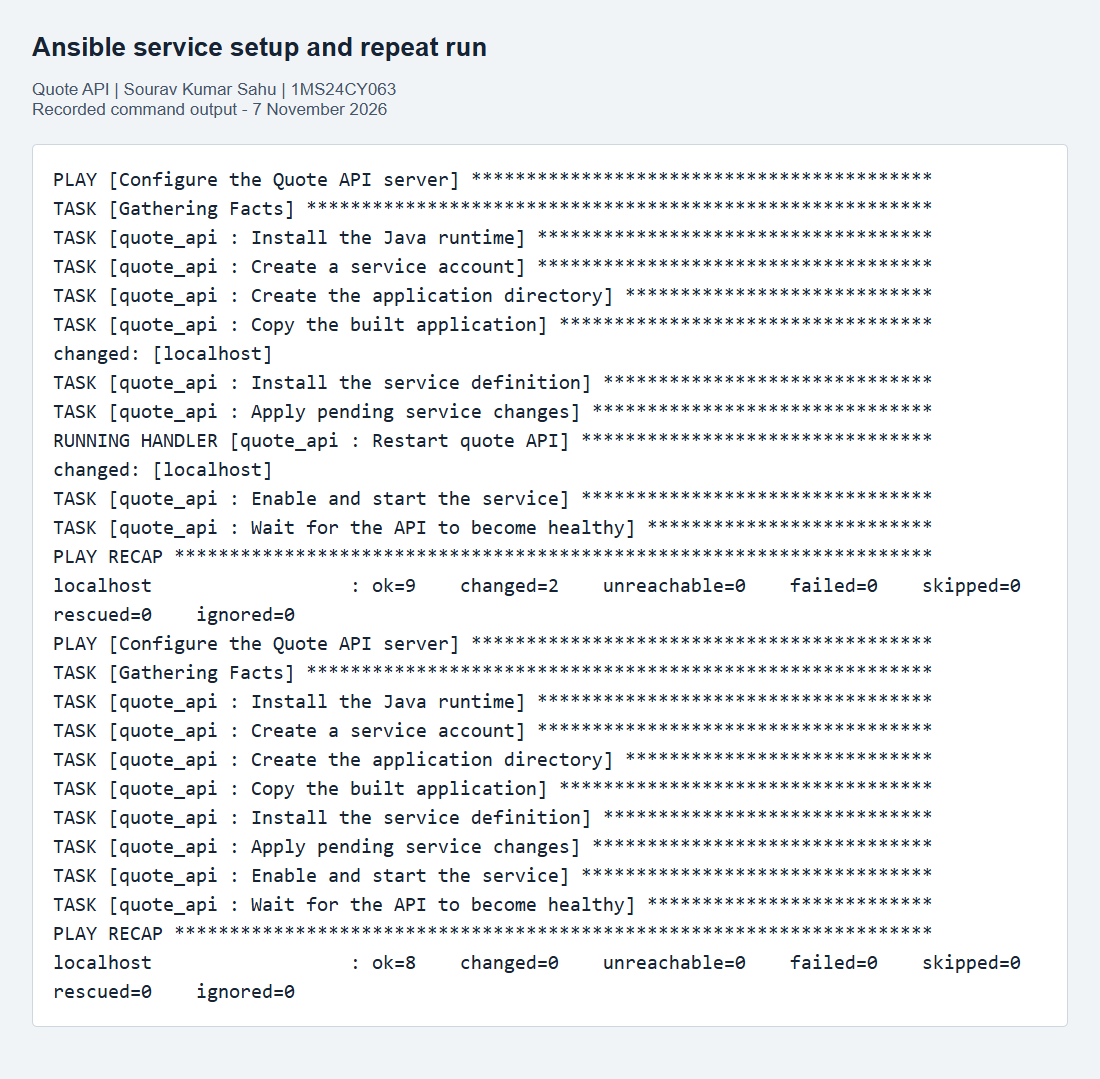
\includegraphics[width=\linewidth,height=0.78\textheight,keepaspectratio]{ansible.png}
\end{center}
\noindent Ansible results: deployment of the final JAR and an unchanged repeat run with zero failures and zero changes.

\clearpage
\begin{center}
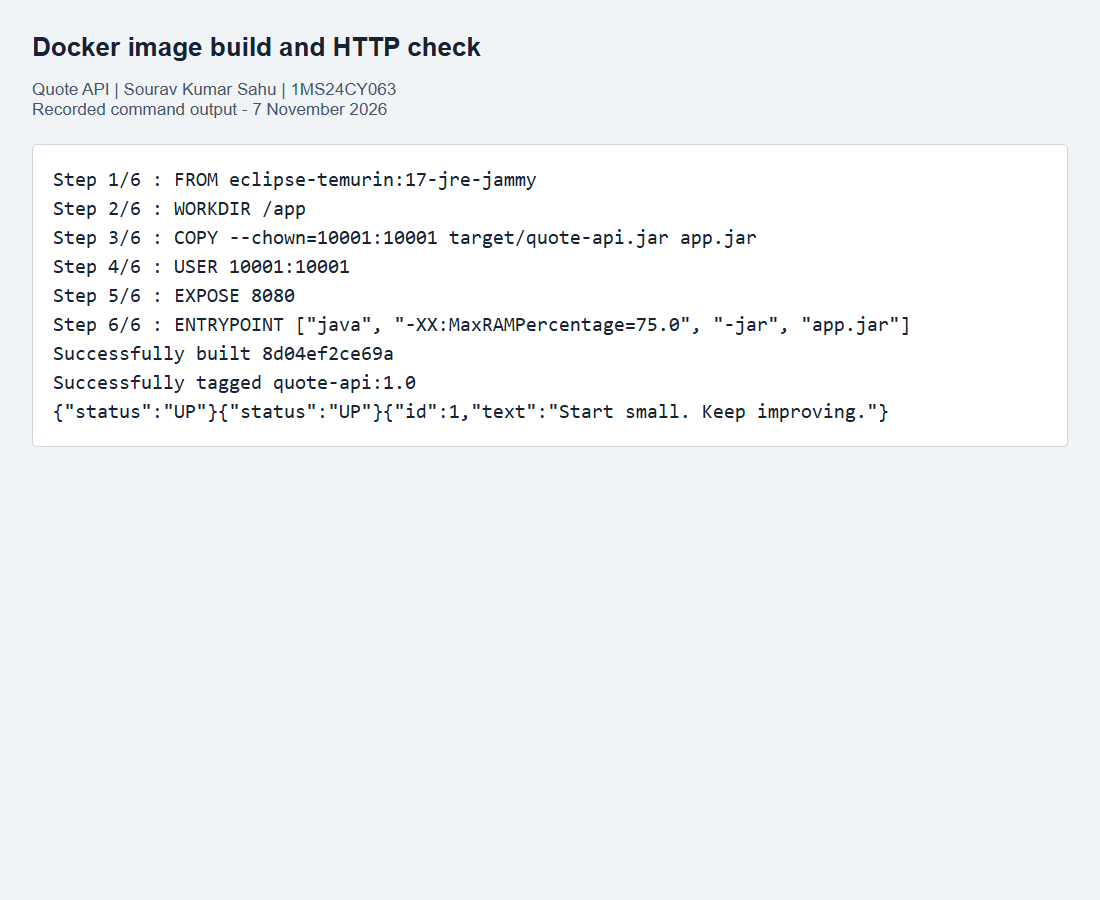
\includegraphics[width=\linewidth,height=0.78\textheight,keepaspectratio]{docker.png}
\end{center}
\noindent Docker verification: the image built successfully and returned the health and quote responses.

\clearpage
\begin{center}
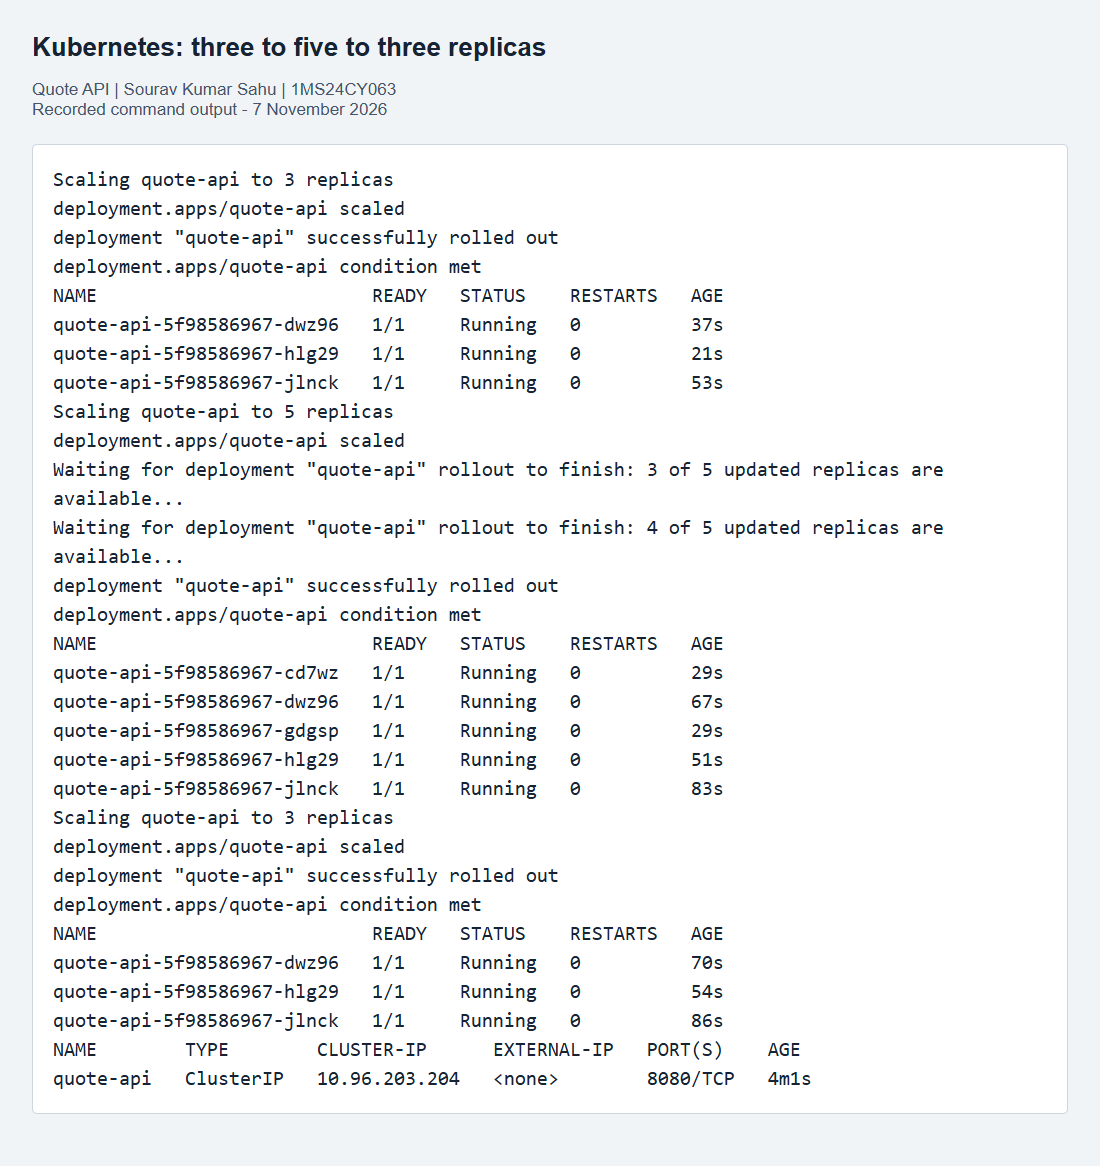
\includegraphics[width=\linewidth,height=0.78\textheight,keepaspectratio]{kubernetes-scaling.png}
\end{center}
\noindent Scaling evidence: three healthy pods, five healthy pods, and three again; the ClusterIP Service remains available.

\clearpage
\begin{center}
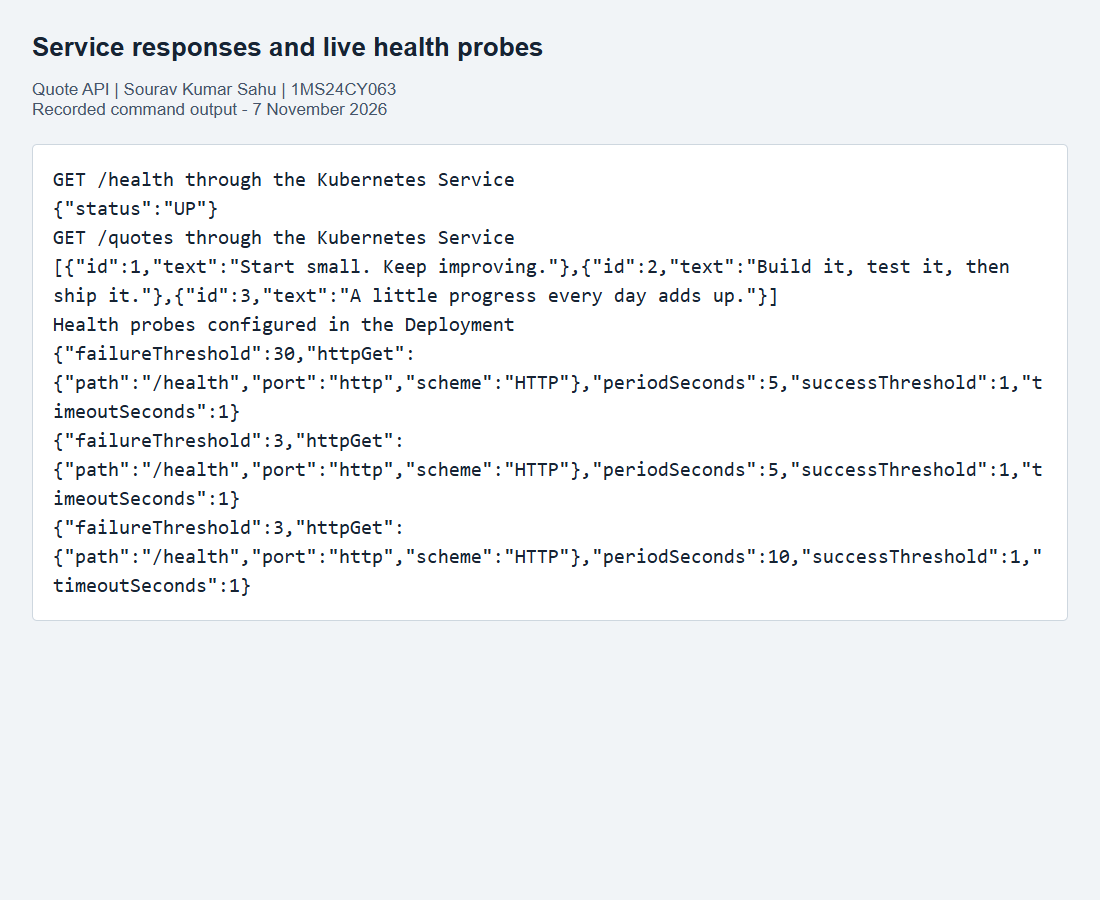
\includegraphics[width=\linewidth,height=0.78\textheight,keepaspectratio]{kubernetes-health.png}
\end{center}
\noindent Service and enhancement evidence: successful HTTP responses and the startup, readiness and liveness probes read from the live Deployment.


\subsection*{Conclusion}
The same small API was installed through repeatable server configuration and then run as a scalable container workload. The zero-change Ansible rerun demonstrates idempotence, while the pod and Service results show how Kubernetes reconciles replica counts without changing the client-facing route. Health probes add a useful distinction between a running process and a pod that is ready to receive requests.

\newpage
\section*{References}
\begin{enumerate}[nosep]
\item Source code and recorded evidence: \url{https://github.com/printf-sourav/DevOps-project}.
\item Official Git documentation: \url{https://git-scm.com/doc}.
\item Maven build lifecycle: \url{https://maven.apache.org/guides/introduction/introduction-to-the-lifecycle.html}.
\item Spring Boot 3.5 requirements: \url{https://docs.spring.io/spring-boot/3.5/system-requirements.html}.
\item Jenkins Pipeline syntax: \url{https://www.jenkins.io/doc/book/pipeline/syntax/}.
\item Jenkins JUnit step: \url{https://www.jenkins.io/doc/pipeline/steps/junit/}.
\item Ansible roles: \url{https://docs.ansible.com/projects/ansible/latest/playbook_guide/playbooks_reuse_roles.html}.
\item Dockerfile reference: \url{https://docs.docker.com/reference/dockerfile/}.
\item Kind quick start: \url{https://kind.sigs.k8s.io/docs/user/quick-start/}.
\item Kubernetes Deployments: \url{https://kubernetes.io/docs/concepts/workloads/controllers/deployment/}.
\item Kubernetes health probes: \url{https://kubernetes.io/docs/tasks/configure-pod-container/configure-liveness-readiness-startup-probes/}.
\end{enumerate}
\end{document}
